% !TEX root = Projektstudie.tex
%Hardware

\section{Hardware}
\label{sec:Hardware}

Kapitel \ref{sec:Hardware} beschreibt die vorhandenen Hardware. Gegliedert ist es in die Teilaspekte Mecanum-Roboter, Meacum-Räder, notwendige Hardwareänderungen und Elektronik.
\subsection{Mecanum-Roboter}
\label{sec:Mecanum-Roboter}

\begin{figure}[H]
\centering
 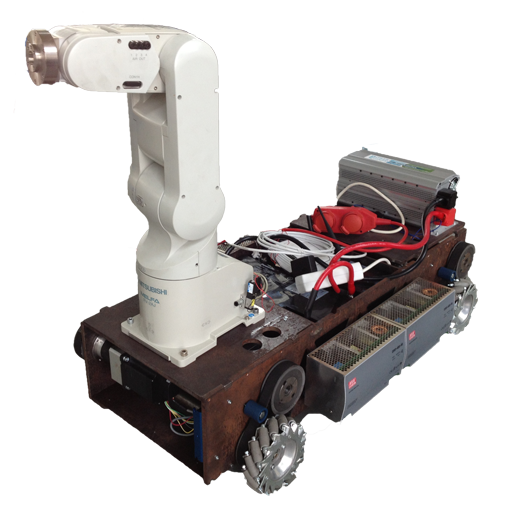
\includegraphics[width=.6\textwidth]{Abbildungen/Roboter} 
\caption[Mecanum-Roboter]{Mecanum-Roboter.}
\label{fig:Roboter}
\end{figure}


Der Mecanum-Roboter ist 1000 mm lang. Er ist mit vier Mecanum-Rädern, die im Rechteck angeordnet sind, ausgestattet. Der Radstand beträgt 775 mm und die Spurbreite beträgt 490 mm. Die Räder haben einen Durchmesser von 115 mm und besitzen jeweils 15 Hilfsrollen. Eine detaillierte Beschreibung folgt im Kapitel \ref{sec:Mecanum-Räder}.

Die Anordnung der Mecanum-Räder und deren Technologie ermöglichen dem Mecanum-Roboter eine omnidirektionale Bewegung. Er kann sich ohne mechanische Lenkung aus jeder Position in jede Richtung fortbewegen.

\subsection{Mecanum-Räder}
\label{sec:Mecanum-Räder}
Das Mecanum Rad wurde 1973 von der schwedischen Firma Mecanum AB entwickelt und bedient unter-schiedliche Anwendungen. Heutige Anwendungsbeispiele sind unter anderem Förderfahrzeuge, fahrerlose Transportfahrzeuge oder Mobilitätshilfe. Auch in der Robotik finden die Allseitenräder immer häufiger Verwendung.
BILD
Abbilung \ref{fig:} zeigt ein Mecanum-Rad des Mecanum-Roboters. Auf dem Umfang des Rades sind 15 tonnen-förmige beschichtete Rollen im Winkel von 45 Grad zu Radachse angebracht. Diese Rollen haben keinen eigenen Antrieb und sind frei drehbar gelagert. Ausschließlich die Rollen haben Kontakt zum Boden.
Jedes Mecanum-Rad wird von einem Schrittmotor angetrieben. Somit sind Drehsinn und Drehzahl für jedes Rad einzeln ansteuerbar. Dieses ist entscheidend für die omnidirektionale Bewegung.
Durch eine individuelle Drehrichtungsauswahl entstehen durch die Hilfsrollen am Untergrund Kraftvektoren in unterschiedliche Richtungen. Die Summe der Vektoren aller Räder bildet die Gesamtbewegungs-richtung oder auch ein Gesamtdrehmoment.

\subsection{Notwendige Hardwareänderung}
Um eine sichere Steuerung zu gewährleisten ist es notwendig die Hardware zu optimieren.
Die Netzanschlussleitung der vier Netzteile wird komplett erneuert. Der Schutzleiter wird angeschlossen wobei auf eine korrekte Anwendung der Zugentlastungen geachtet wird. Die Erdung des Schutzleiters wird über Erdungsklemmen auf das Fahrzeuggehäuse gelegt.
Vor der Hardwareänderung sind je zwei Motortreiberkarten über einen separaten CAN-Bus von der ver-bauten SPS angesprochen worden. Um einen Betrieb sowohl über den Arduino als auch über die SPS zu ermöglichen werden alle Komponenten auf einen CAN-Bus zusammengelegt, die Motortreiberkarten umadressiert und die 120 Ohm Abschlusswiderstände in den äußersten Steckern eingelötet.
Da die Steckerbelegung des Arduino-CAN-Shield von der ISO 11 898 Norm abweicht, wurde der entsprechende Stecker der Busleitung angepasst. Ein weiterer Stecker zur Diagnose der CAN-Bus-Signale via PC wird angelötet.
Die verwendete Schraubenlänge zur Befestigung der Mecanum-Räder war ungenügend. Alle vier Mecanum - Räder sind nun mit je drei M5 Schrauben befestigt.